\part{Second-Order-DEs}
\lecture{Second Order DEs}{Second-Order-DEs}
\section{Second Order DEs}

\title{Ordinary Differential Equations}
\subtitle{Math 232 - Linear, Constant Coefficient ODEs}
\date{23 September 2013}

\begin{frame}
  \titlepage
\end{frame}

\begin{frame}
  \frametitle{Outline}
  \tableofcontents[currentsection ]
\end{frame}


\subsection{Second Order DEs}


\iftoggle{clicker}{%
\begin{frame}
  \frametitle{Clicker Quiz}

      \ifnum\value{clickerQuiz}=1{%

        \vfill

        Determine the value of $z_1 + \bar{z}_1$ where $z_1=3-2i$.

        \vfill

        \begin{tabular}{ll}
          A: & 3 \\
          B: & 6 \\
          C: & 4i \\
          D: & -4i
        \end{tabular}


        \vfill

      }\fi

      \ifnum\value{clickerQuiz}=2{%

        \vfill

        Determine the value of $z_1 - \bar{z}_1$ where $z_1=2+4i$.

        \vfill

        \begin{tabular}{ll}
          A: & -4 \\
          B: & 4 \\
          C: & 8i \\
          D: & -8i
        \end{tabular}


        \vfill

     }\fi
   
     \ifnum\value{clickerQuiz}=3{%

        \vfill

        Determine the value of $z_1 - \bar{z}_1$ where $z_1=7+2i$.

        \vfill

        \begin{tabular}{ll}
          A: & -14 \\
          B: & -14 \\
          C: & 4i \\
          D: & -4i
        \end{tabular}


        \vfill


    }\fi
  

\end{frame}
}



\begin{frame}
  \frametitle{Second Order Equations}

  The General, Constant Coefficient, Linear, Second Order Homogeneous
  Differential Equation:
  \begin{eqnarray*}
    {\color{red}m} x'' + {\color{red}b} x' + {\color{red}k}x & = & 0.
  \end{eqnarray*}
  The parameters {\color{red}$m$}, {\color{red}$b$}, and {\color{red}$k$} are constants.

  This is also called the ``Damped Harmonic Oscillator.''

\end{frame}

\subsection{Horizontal Spring/Mass Systems}

\begin{frame}
  \frametitle{Horizontal Spring/Mass System}

  \only<1>{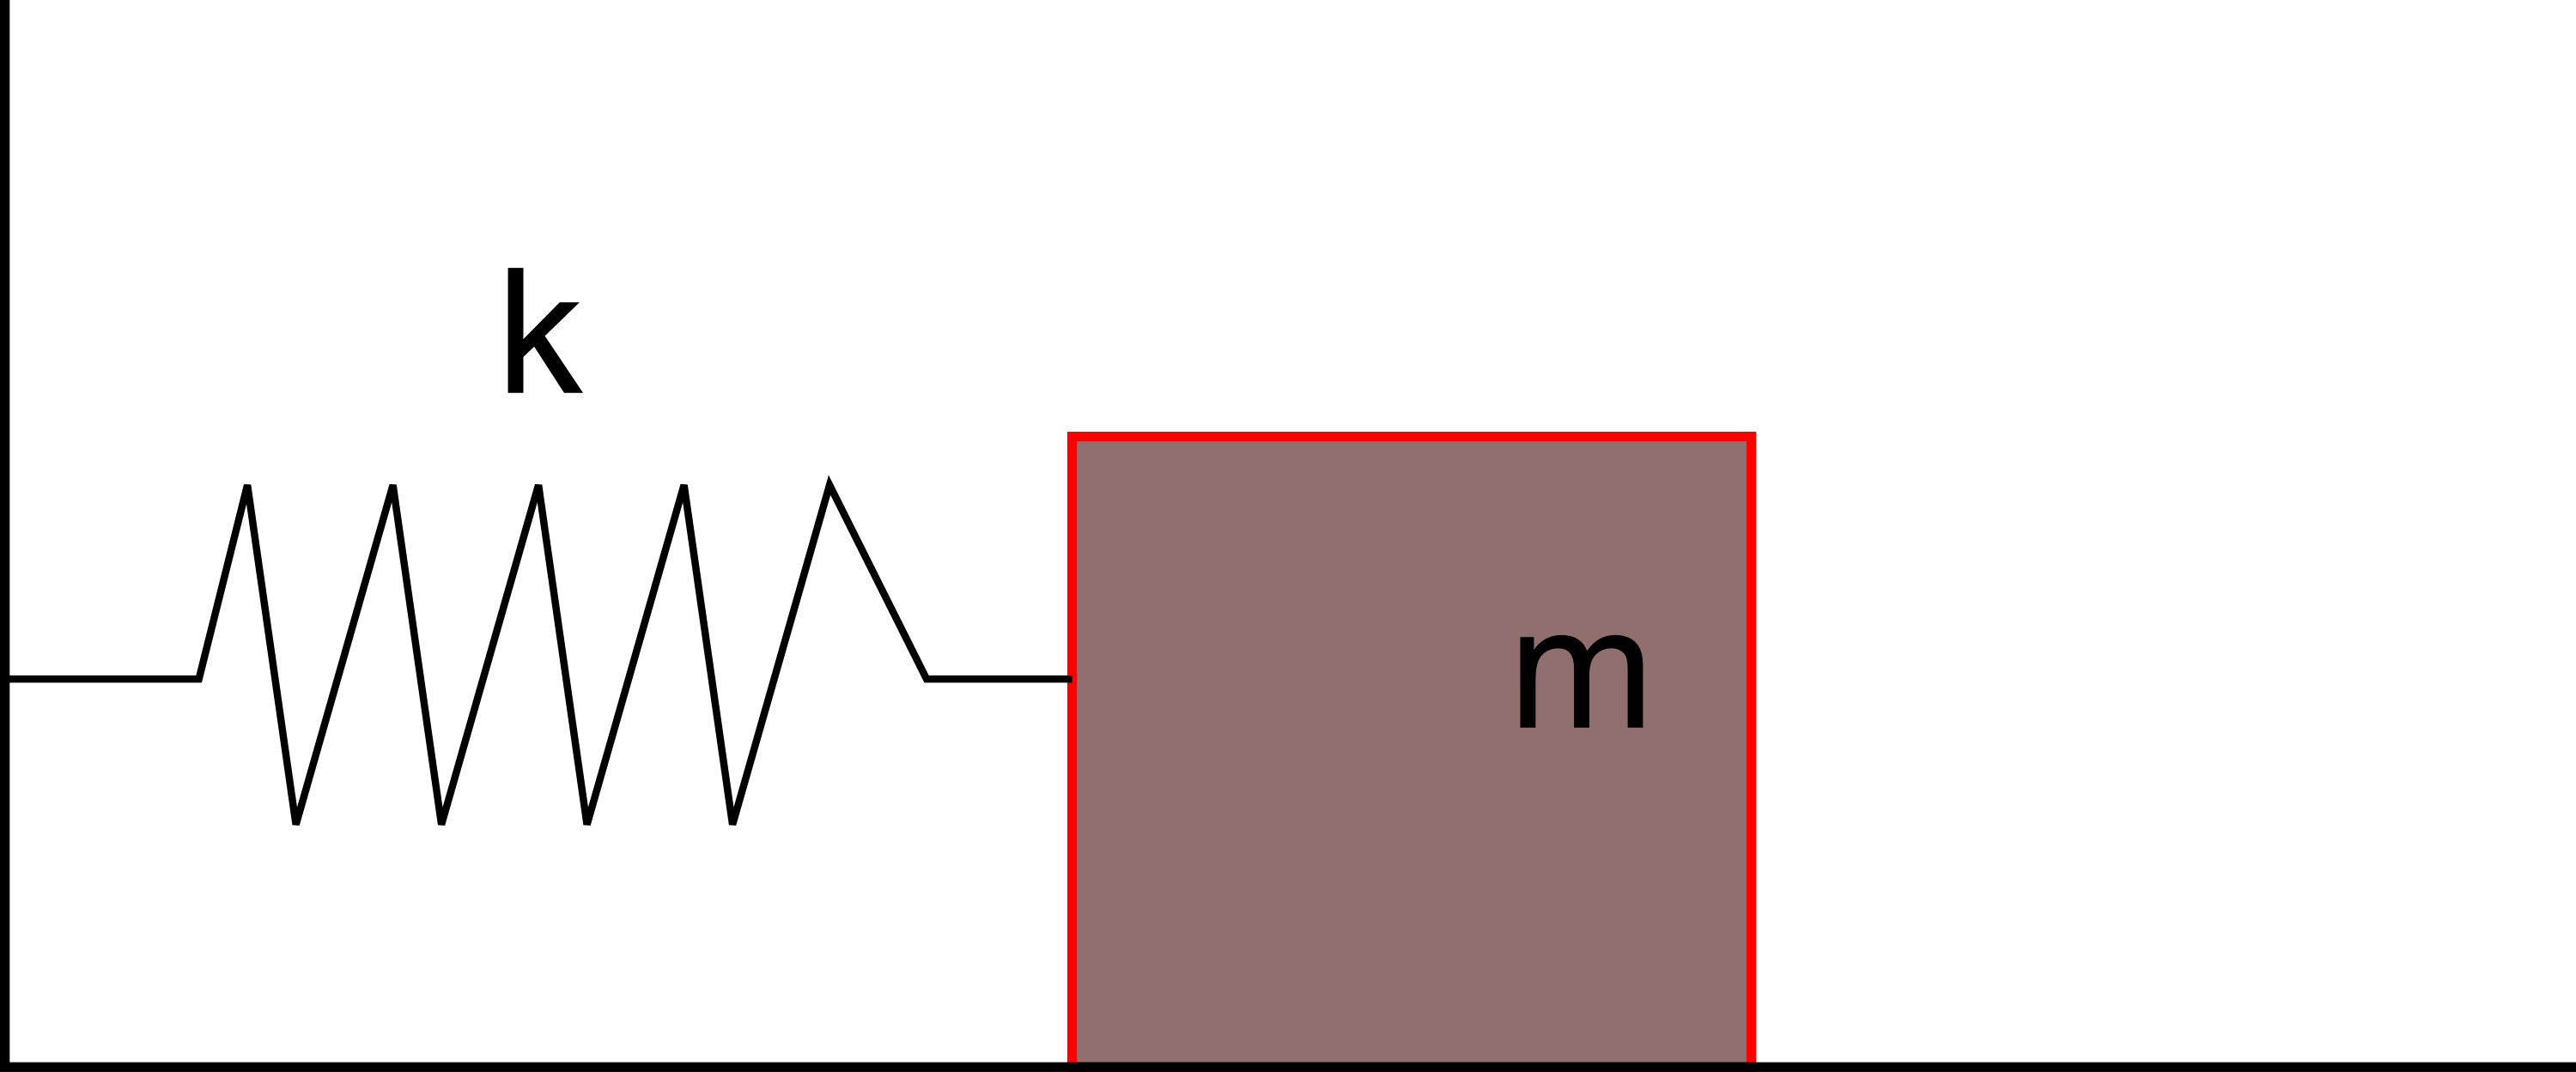
\includegraphics[width=6cm]{img/springMassStatic}}
  \only<2>{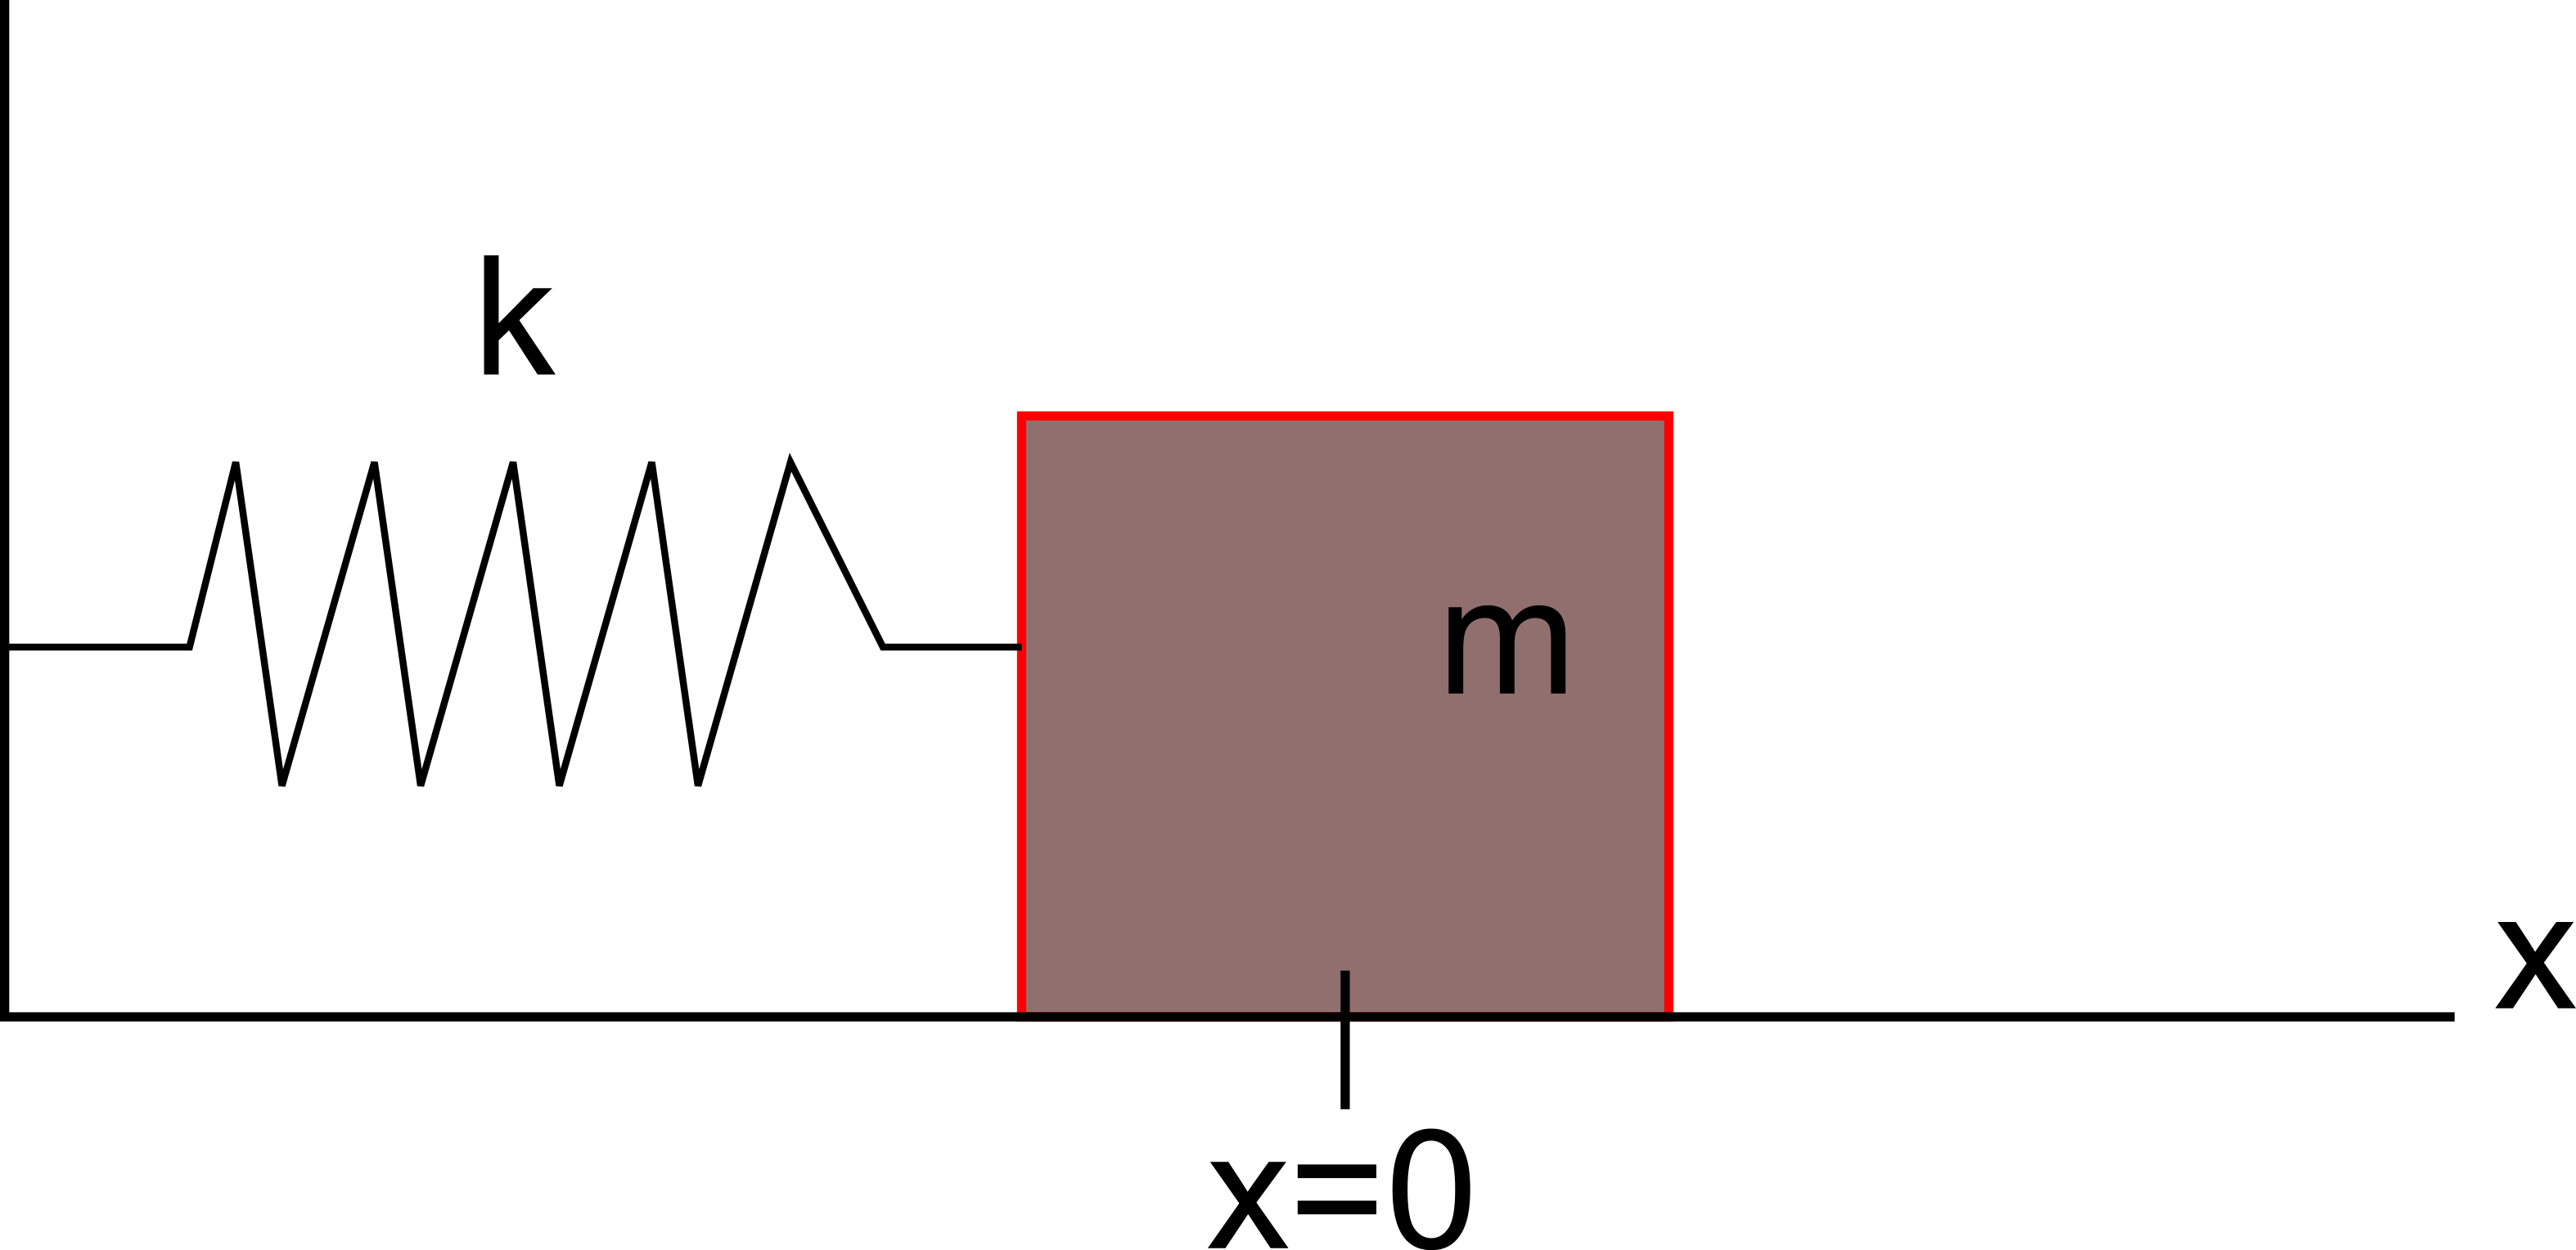
\includegraphics[width=6cm]{img/springMassStaticCoordinates}}
  \only<3>{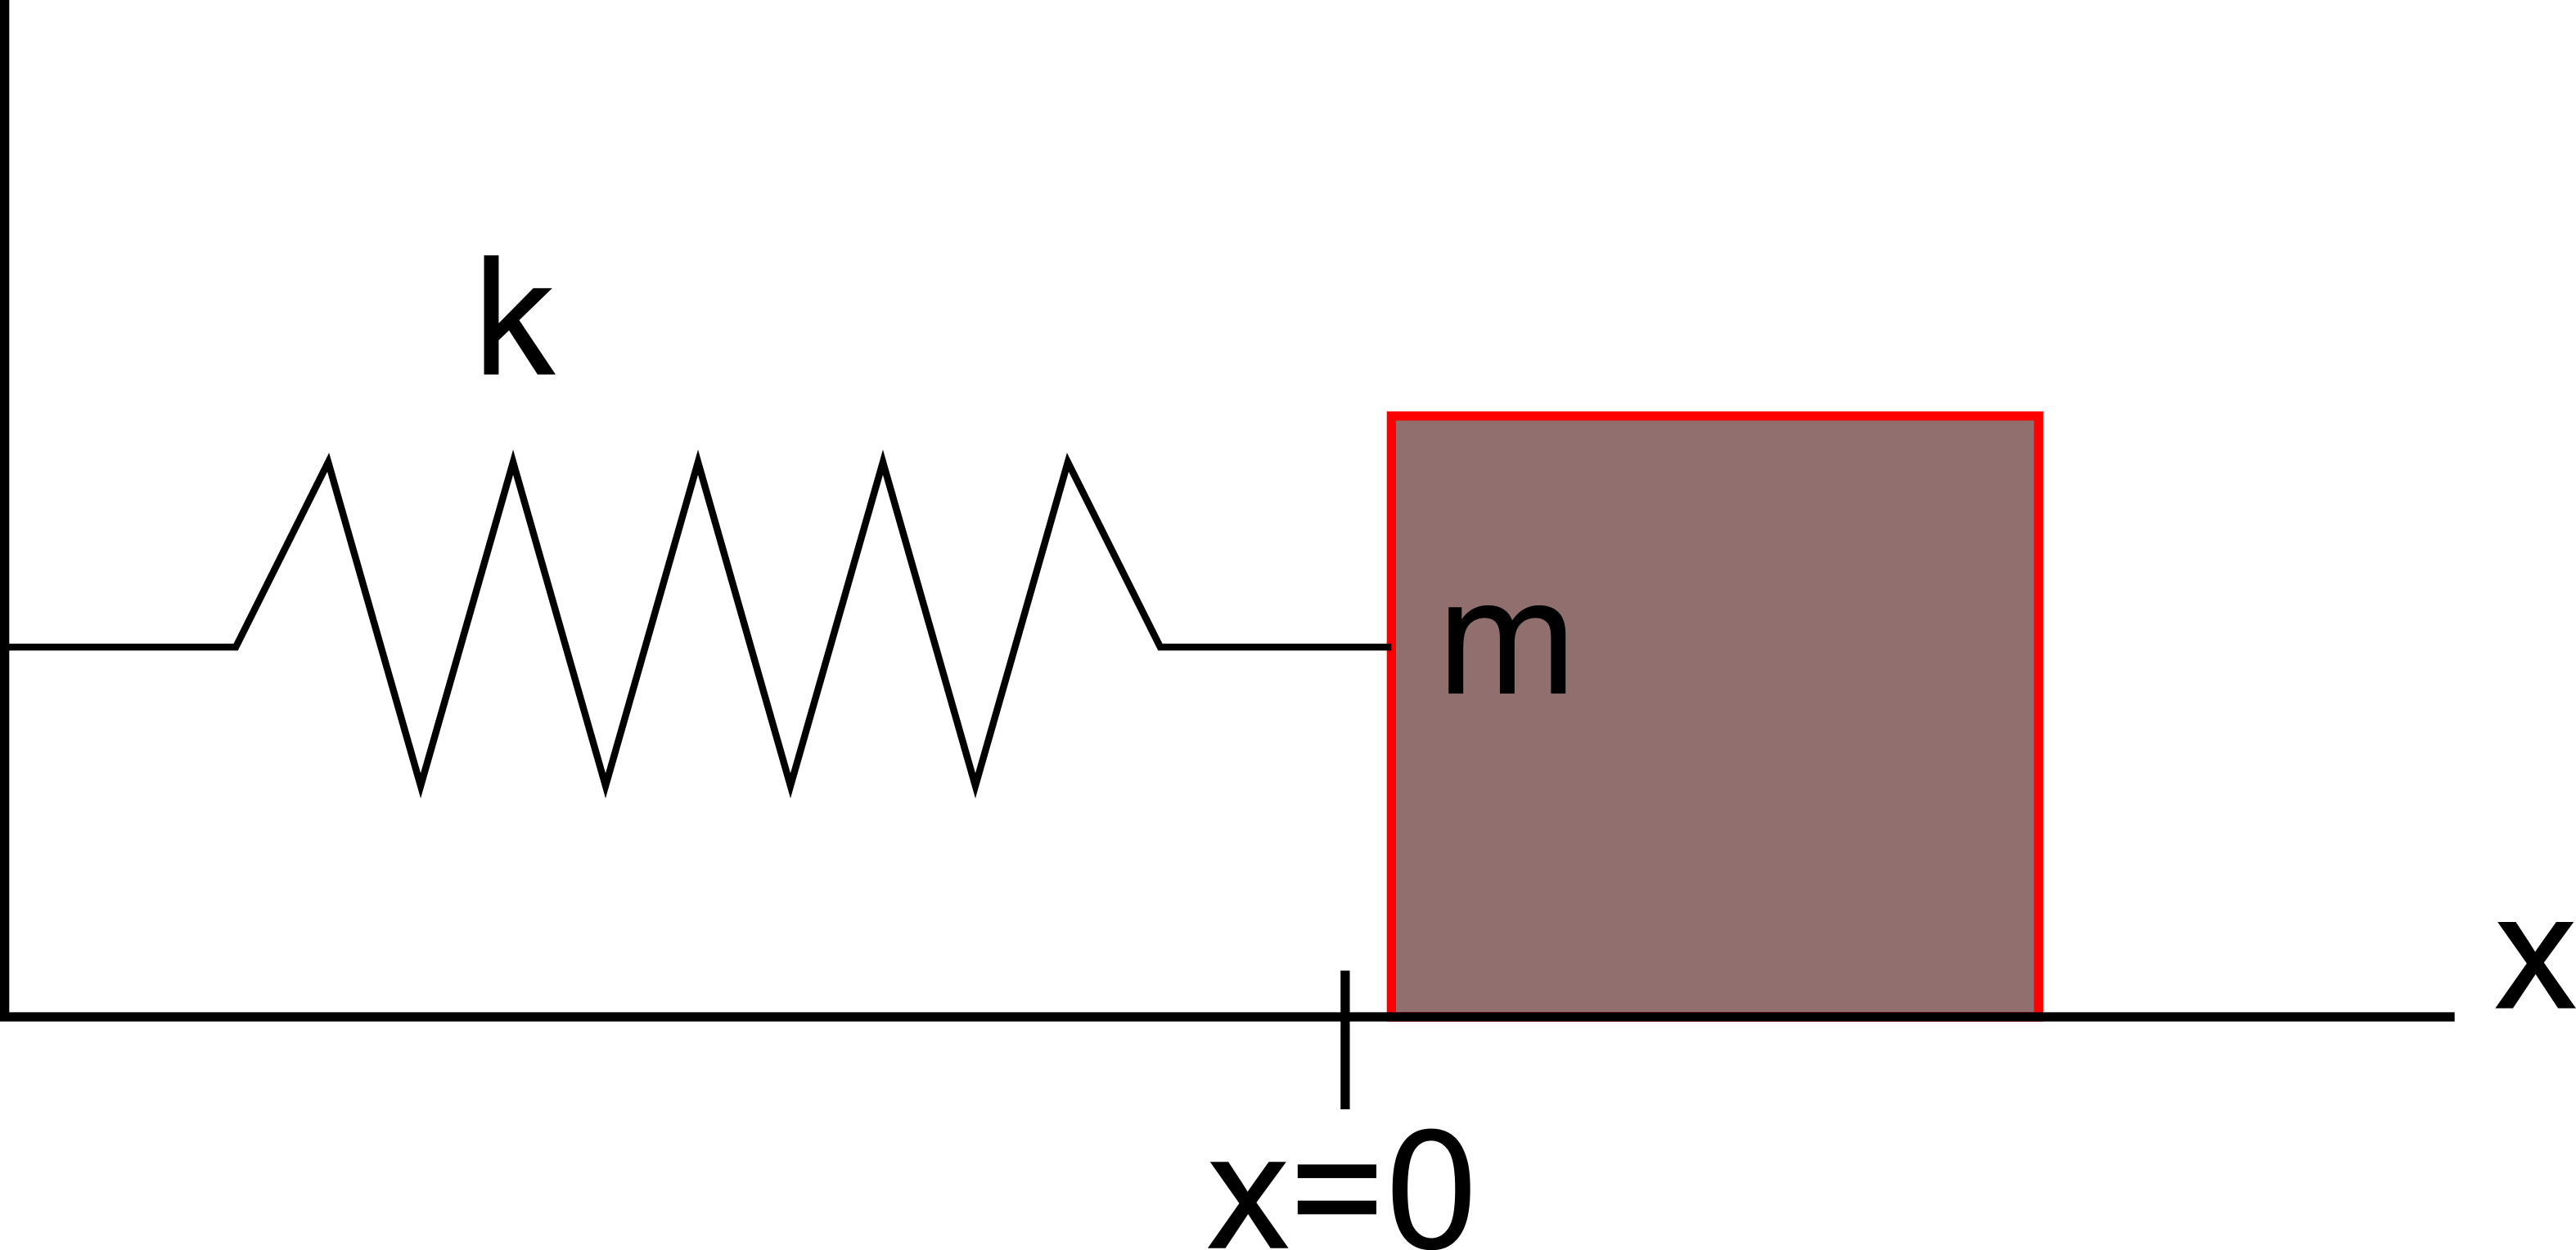
\includegraphics[width=6cm]{img/springMassDynamic}}
  \only<4->{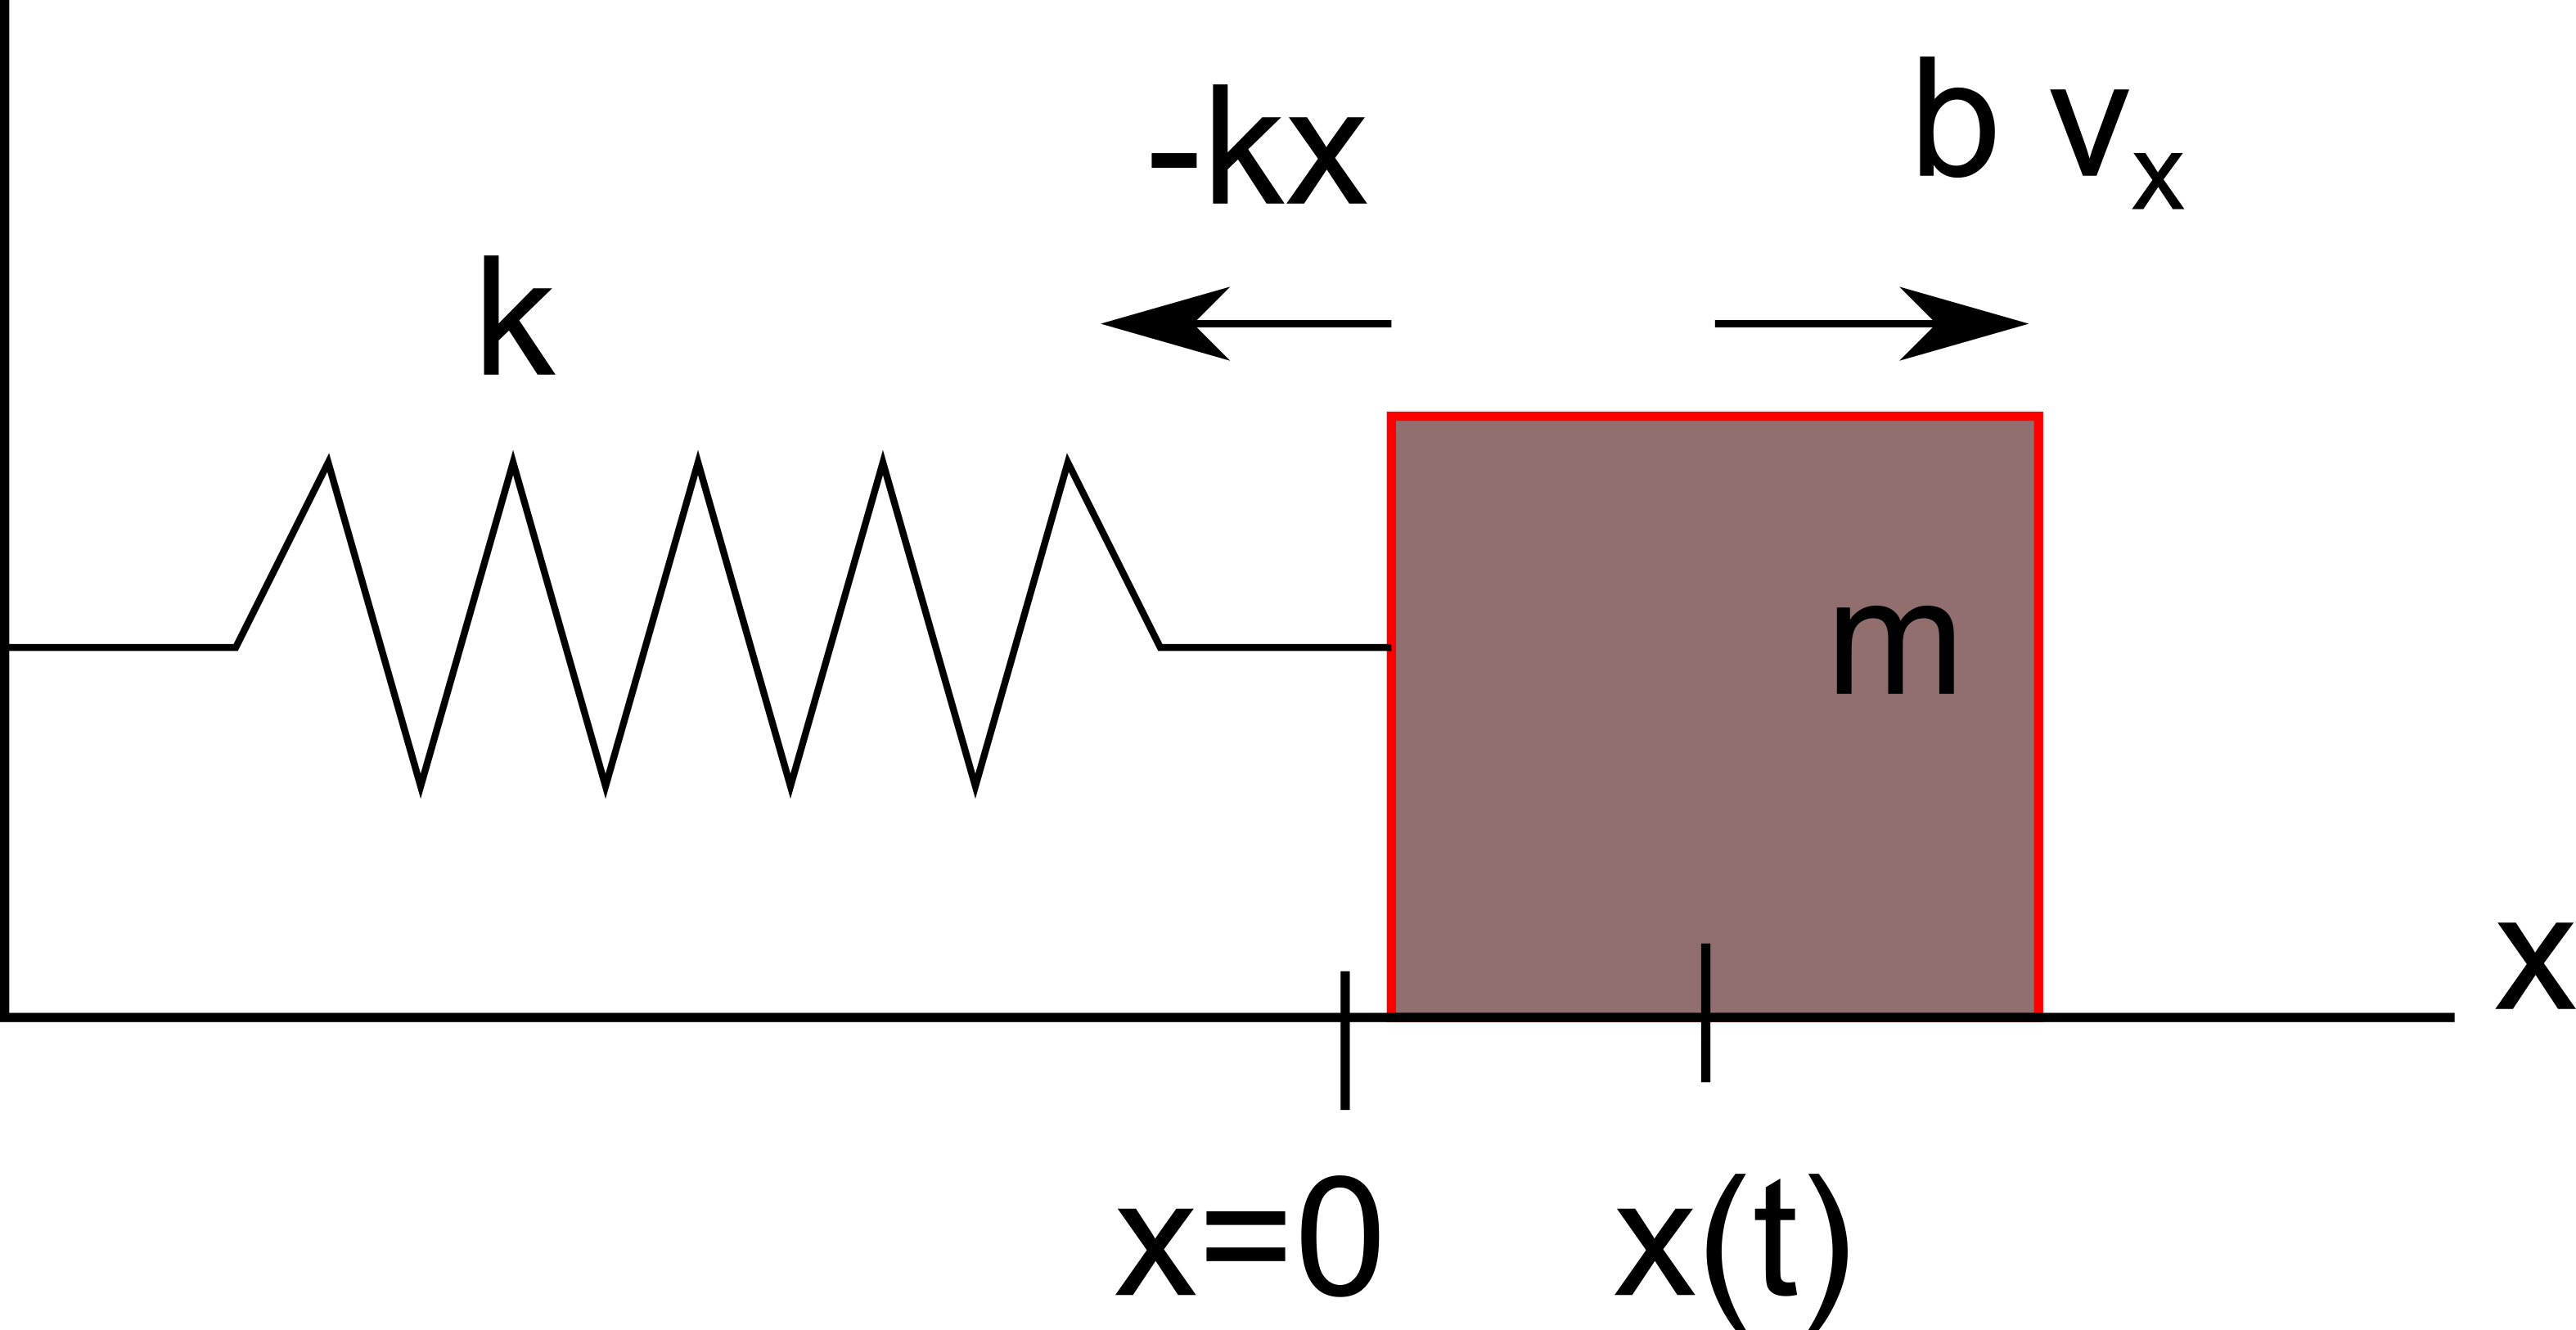
\includegraphics[width=6cm]{img/springMassDynamicVectors}}

  \uncover<4->{%
    Newton's Second Law:
    \begin{eqnarray*}
      \frac{d}{dt} \lp m \vec{v} \rp & = & \sum_i \vec{F}_i \\
      & = & -kx - bv_x 
    \end{eqnarray*}
    or
    \begin{eqnarray*}
      mx'' + bx' + kx & = & 0.
    \end{eqnarray*}

    If $b=0$ it is an ``\textbf{undamped''} system, otherwise it is ``\textbf{damped}.''
  }

\end{frame}


\begin{frame}
  \frametitle{Example}

  A mass of 2 kg is resting on an horizontal table and is attached to
  a linear spring which has a spring constant of 3 N/m. The force of
  friction is 1.5 times the velocity. The block is pulled to the left
  0.5m and let go from rest. Find the governing equation.

  \uncover<2->
  {
    \begin{eqnarray*}
      2 x'' + 1.5 x' + 3x & = & 0, \\
      x(0) & = & -.5m, \\
      x'(0) & = & 0 m/s.
    \end{eqnarray*}

    Need two initial conditions!
  }

\end{frame}


\begin{frame}
  \frametitle{Lots of variations}

  \begin{itemize}
  \item Could say that the spring stretched .25 m when 2N is applied.
  \item Could say that the force of friction is 0.5N when it is moving
    .3 m/s. 
  \end{itemize}

  See example on p. 197.

\end{frame}

\subsection{Undamped Systems}

\iftoggle{clicker}{%
\begin{frame}
  \frametitle{Clicker Quiz}

      \ifnum\value{clickerQuiz}=1{%

        \vfill

        Suppose that the spring/mass system has no friction,
        $b=0$, 
        \begin{eqnarray*}
          m x'' + kx & = & 0.
        \end{eqnarray*}        
        What kind of behavior do you expect?

        \vfill

        \begin{tabular}{ll}
          A: & Infinite, perfect oscillations until the end of time. \\
             & (or the end of today's class whichever comes first)  \\
          B: & Oscillations slowly dieing out.  \\
          C: & Oscillations with slow but steady decay \\
          D  & Oscillations with exponential decay
        \end{tabular}


        \vfill

      }\fi

      \ifnum\value{clickerQuiz}=2{%

        \vfill
        Suppose that the spring/mass system has no friction,
        $b=0$, 
        \begin{eqnarray*}
          m x'' + kx & = & 0.
        \end{eqnarray*}        
        What kind of behavior do you expect?

        \vfill

        \begin{tabular}{ll}
          A: & Infinite, perfect oscillations until the end of time. \\
             & (or the end of today's class whichever comes first)  \\
          B: & Oscillations slowly dieing out.  \\
          C: & Oscillations with slow but steady decay \\
          D  & Oscillations with exponential decay
        \end{tabular}


        \vfill

     }\fi
   
     \ifnum\value{clickerQuiz}=3{%
        Suppose that the spring/mass system has no friction,
        $b=0$,
        \begin{eqnarray*}
          m x'' + kx & = & 0.
        \end{eqnarray*}
        What kind of behavior do you expect?

        \vfill

        \begin{tabular}{ll}
          A: & Infinite, perfect oscillations until the end of time. \\
             & (or the end of today's class whichever comes first)  \\
          B: & Oscillations slowly dieing out.  \\
          C: & Oscillations with slow but steady decay \\
          D  & Oscillations with exponential decay
        \end{tabular}


        \vfill

    }\fi
  

\end{frame}
}



\begin{frame}
  \frametitle{Special Case}

  No friction, $b=0$: \textit{(Use your intuition!)} 
  \begin{eqnarray*}
    m x'' + kx & = & 0.
  \end{eqnarray*}

  \uncover<2->
  {
    Assume solutions of the form 
    \begin{eqnarray*}
      x & = & C_1 \cos(\redText{\omega} t) + C_2 \sin(\redText{\omega} t) \\
      \uncover<3->
      {
        x' & = & -\redText{\omega} C_1 \sin(\redText{\omega} t) + \redText{\omega} C_2 \cos(\redText{\omega} t) \\
      }
      \uncover<4->
      {
        x'' & = & -\redText{\omega}^2 C_1 \cos(\redText{\omega} t) - \redText{\omega}^2 C_2 \sin(\redText{\omega} t) \\
      }
    \end{eqnarray*}
  }

\end{frame}



\begin{frame}
  \frametitle{Special Case}

  No friction, $b=0$:
  \begin{eqnarray*}
    m x'' + kx & = & 0.
  \end{eqnarray*}

  \uncover<2->
  {
    \begin{eqnarray*}
      0 & = & mx''+kx \\
        & = & - m\redText{\omega}^2 C_1 \cos(\redText{\omega} t) - m\redText{\omega}^2 C_2 \sin(\redText{\omega} t) \\
        &   & + k C_1 \cos(\redText{\omega} t) + k C_2 \sin(\redText{\omega} t)\\
        & = & \lp -m \redText{\omega}^2 + k \rp C_1 \cos(\redText{\omega} t) +
              \lp -m \redText{\omega}^2 + k \rp C_2 \sin(\redText{\omega} t)
    \end{eqnarray*}
  }

  \uncover<3->
  {
    \begin{eqnarray*}
      \Rightarrow \redText{\omega} & = & \pm \sqrt{\frac{k}{m}}.
    \end{eqnarray*}
  }

  \vfill

\end{frame}


\begin{frame}
  \frametitle{Special Case}

  No friction, $b=0$:
  \begin{eqnarray*}
    m x'' + kx & = & 0.
  \end{eqnarray*}

  \begin{eqnarray*}
    x & = & C_1 \cos\lp\sqrt{\frac{k}{m}} t\rp +
    C_2 \sin\lp\sqrt{\frac{k}{m}} t\rp \\
    & = & A \cdot \cos\lp \sqrt{\frac{k}{m}} t - \delta \rp.
  \end{eqnarray*}

  Period = \blueText{T},
  \begin{eqnarray*}
    \sqrt{\frac{k}{m}} \blueText{T} & = & 2\pi, \\
    \Rightarrow \blueText{T} & = & 2 \pi \sqrt{\frac{m}{k}}.
  \end{eqnarray*}

\end{frame}


\begin{frame}
  \frametitle{Example}

  An horizontal spring/mass system is to be constructed using a 2 kg
  mass. What spring constant should be used so that it oscillates at 3
  oscillations per second?

  \begin{eqnarray*}
    2 x'' + \redText{k}x & = & 0 \\
    x & = & A \cdot \cos\lp \sqrt{\frac{\redText{k}}{2}} t - \delta \rp \\
  \end{eqnarray*}

  \uncover<2->
  {
    3 oscillations per second means that
    \begin{eqnarray*}
      \sqrt{\frac{\redText{k}}{2}} \lp \frac{1}{3} \rp & = & 2 \pi, \\
      \redText{k} & = & 72 \pi^2~\mathrm{N/m}.
    \end{eqnarray*}
  }

\end{frame}

\subsection{RCL Circuits}

\begin{frame}
  \frametitle{RCL Circuit}

  See pp. 202-204 for more information about LRC circuits.

  \begin{columns}
    \column{.5\textwidth}
    % Graphic for TeX using PGF
% Title: /home/black/write/class/de/math232-12/ODE-Recitation-Activities/notes/img/LRCcircuit.dia
% Creator: Dia v0.97.2
% CreationDate: Wed Sep 18 10:33:40 2013
% For: black
% \usepackage{tikz}
% The following commands are not supported in PSTricks at present
% We define them conditionally, so when they are implemented,
% this pgf file will use them.
\ifx\du\undefined
  \newlength{\du}
\fi
\setlength{\du}{15\unitlength}
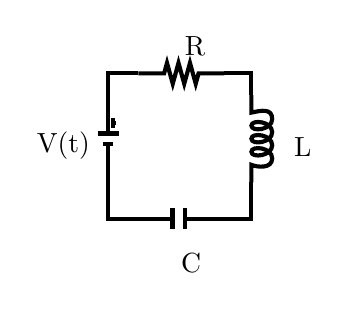
\begin{tikzpicture}
\pgftransformxscale{0.500000}
\pgftransformyscale{-0.500000}
\definecolor{dialinecolor}{rgb}{0.000000, 0.000000, 0.000000}
\pgfsetstrokecolor{dialinecolor}
\definecolor{dialinecolor}{rgb}{1.000000, 1.000000, 1.000000}
\pgfsetfillcolor{dialinecolor}
\pgfsetlinewidth{0.100000\du}
\pgfsetdash{}{0pt}
\pgfsetdash{}{0pt}
\pgfsetbuttcap
\pgfsetmiterjoin
\pgfsetlinewidth{0.100000\du}
\pgfsetbuttcap
\pgfsetmiterjoin
\pgfsetdash{}{0pt}
\definecolor{dialinecolor}{rgb}{0.000000, 0.000000, 0.000000}
\pgfsetstrokecolor{dialinecolor}
\draw (2.900000\du,9.550000\du)--(2.900000\du,10.800000\du);
\pgfsetbuttcap
\pgfsetmiterjoin
\pgfsetdash{}{0pt}
\definecolor{dialinecolor}{rgb}{0.000000, 0.000000, 0.000000}
\pgfsetstrokecolor{dialinecolor}
\draw (2.400000\du,10.800000\du)--(3.400000\du,10.800000\du);
\pgfsetbuttcap
\pgfsetmiterjoin
\pgfsetdash{}{0pt}
\definecolor{dialinecolor}{rgb}{0.000000, 0.000000, 0.000000}
\pgfsetstrokecolor{dialinecolor}
\draw (2.650000\du,11.300000\du)--(3.150000\du,11.300000\du);
\pgfsetbuttcap
\pgfsetmiterjoin
\pgfsetdash{}{0pt}
\definecolor{dialinecolor}{rgb}{0.000000, 0.000000, 0.000000}
\pgfsetstrokecolor{dialinecolor}
\draw (3.150000\du,10.050000\du)--(3.150000\du,10.550000\du);
\pgfsetbuttcap
\pgfsetmiterjoin
\pgfsetdash{}{0pt}
\definecolor{dialinecolor}{rgb}{0.000000, 0.000000, 0.000000}
\pgfsetstrokecolor{dialinecolor}
\draw (3.025000\du,10.300000\du)--(3.275000\du,10.300000\du);
\pgfsetbuttcap
\pgfsetmiterjoin
\pgfsetdash{}{0pt}
\definecolor{dialinecolor}{rgb}{0.000000, 0.000000, 0.000000}
\pgfsetstrokecolor{dialinecolor}
\draw (2.900000\du,11.300000\du)--(2.900000\du,12.550000\du);
\pgfsetlinewidth{0.100000\du}
\pgfsetdash{}{0pt}
\pgfsetdash{}{0pt}
\pgfsetbuttcap
\pgfsetmiterjoin
\pgfsetlinewidth{0.100000\du}
\pgfsetbuttcap
\pgfsetmiterjoin
\pgfsetdash{}{0pt}
\definecolor{dialinecolor}{rgb}{0.000000, 0.000000, 0.000000}
\pgfsetstrokecolor{dialinecolor}
\draw (4.350000\du,7.900000\du)--(5.595000\du,7.900000\du)--(5.733333\du,7.400000\du)--(6.010000\du,8.400000\du)--(6.286667\du,7.400000\du)--(6.563333\du,8.400000\du)--(6.840000\du,7.400000\du)--(7.116667\du,8.400000\du)--(7.255000\du,7.900000\du)--(8.500000\du,7.900000\du);
\pgfsetlinewidth{0.100000\du}
\pgfsetdash{}{0pt}
\pgfsetdash{}{0pt}
\pgfsetbuttcap
\pgfsetmiterjoin
\pgfsetlinewidth{0.100000\du}
\pgfsetbuttcap
\pgfsetmiterjoin
\pgfsetdash{}{0pt}
\definecolor{dialinecolor}{rgb}{0.000000, 0.000000, 0.000000}
\pgfsetstrokecolor{dialinecolor}
\pgfpathmoveto{\pgfpoint{9.800000\du}{8.950000\du}}
\pgfpathlineto{\pgfpoint{9.800000\du}{9.790000\du}}
\pgfpathcurveto{\pgfpoint{10.300000\du}{9.685000\du}}{\pgfpoint{10.800000\du}{9.580000\du}}{\pgfpoint{10.800000\du}{10.105000\du}}
\pgfpathcurveto{\pgfpoint{10.800000\du}{10.630000\du}}{\pgfpoint{9.800000\du}{10.735000\du}}{\pgfpoint{9.800000\du}{10.420000\du}}
\pgfpathcurveto{\pgfpoint{9.800000\du}{10.105000\du}}{\pgfpoint{10.800000\du}{10.210000\du}}{\pgfpoint{10.800000\du}{10.735000\du}}
\pgfpathcurveto{\pgfpoint{10.800000\du}{11.260000\du}}{\pgfpoint{9.800000\du}{11.365000\du}}{\pgfpoint{9.800000\du}{11.050000\du}}
\pgfpathcurveto{\pgfpoint{9.800000\du}{10.735000\du}}{\pgfpoint{10.800000\du}{10.840000\du}}{\pgfpoint{10.800000\du}{11.365000\du}}
\pgfpathcurveto{\pgfpoint{10.800000\du}{11.890000\du}}{\pgfpoint{9.800000\du}{11.995000\du}}{\pgfpoint{9.800000\du}{11.680000\du}}
\pgfpathcurveto{\pgfpoint{9.800000\du}{11.365000\du}}{\pgfpoint{10.800000\du}{11.470000\du}}{\pgfpoint{10.800000\du}{11.995000\du}}
\pgfpathcurveto{\pgfpoint{10.800000\du}{12.520000\du}}{\pgfpoint{10.050000\du}{12.415000\du}}{\pgfpoint{9.800000\du}{12.310000\du}}
\pgfpathlineto{\pgfpoint{9.800000\du}{13.150000\du}}
\pgfusepath{stroke}
\pgfsetlinewidth{0.100000\du}
\pgfsetdash{}{0pt}
\pgfsetdash{}{0pt}
\pgfsetbuttcap
\pgfsetmiterjoin
\pgfsetlinewidth{0.100000\du}
\pgfsetbuttcap
\pgfsetmiterjoin
\pgfsetdash{}{0pt}
\definecolor{dialinecolor}{rgb}{0.000000, 0.000000, 0.000000}
\pgfsetstrokecolor{dialinecolor}
\draw (4.800000\du,14.900000\du)--(6.000000\du,14.900000\du);
\pgfsetbuttcap
\pgfsetmiterjoin
\pgfsetdash{}{0pt}
\definecolor{dialinecolor}{rgb}{0.000000, 0.000000, 0.000000}
\pgfsetstrokecolor{dialinecolor}
\draw (6.000000\du,14.400000\du)--(6.000000\du,15.400000\du);
\pgfsetbuttcap
\pgfsetmiterjoin
\pgfsetdash{}{0pt}
\definecolor{dialinecolor}{rgb}{0.000000, 0.000000, 0.000000}
\pgfsetstrokecolor{dialinecolor}
\draw (6.600000\du,14.400000\du)--(6.600000\du,15.400000\du);
\pgfsetbuttcap
\pgfsetmiterjoin
\pgfsetdash{}{0pt}
\definecolor{dialinecolor}{rgb}{0.000000, 0.000000, 0.000000}
\pgfsetstrokecolor{dialinecolor}
\draw (6.600000\du,14.900000\du)--(7.800000\du,14.900000\du);
\pgfsetlinewidth{0.100000\du}
\pgfsetdash{}{0pt}
\pgfsetdash{}{0pt}
\pgfsetmiterjoin
\pgfsetbuttcap
{
\definecolor{dialinecolor}{rgb}{0.000000, 0.000000, 0.000000}
\pgfsetfillcolor{dialinecolor}
% was here!!!
{\pgfsetcornersarced{\pgfpoint{0.000000\du}{0.000000\du}}\definecolor{dialinecolor}{rgb}{0.000000, 0.000000, 0.000000}
\pgfsetstrokecolor{dialinecolor}
\draw (8.500000\du,7.900000\du)--(9.800000\du,7.900000\du)--(9.800000\du,8.950000\du);
}}
\pgfsetlinewidth{0.100000\du}
\pgfsetdash{}{0pt}
\pgfsetdash{}{0pt}
\pgfsetmiterjoin
\pgfsetbuttcap
{
\definecolor{dialinecolor}{rgb}{0.000000, 0.000000, 0.000000}
\pgfsetfillcolor{dialinecolor}
% was here!!!
{\pgfsetcornersarced{\pgfpoint{0.000000\du}{0.000000\du}}\definecolor{dialinecolor}{rgb}{0.000000, 0.000000, 0.000000}
\pgfsetstrokecolor{dialinecolor}
\draw (2.900000\du,9.550000\du)--(2.900000\du,7.900000\du)--(4.350000\du,7.900000\du);
}}
\pgfsetlinewidth{0.100000\du}
\pgfsetdash{}{0pt}
\pgfsetdash{}{0pt}
\pgfsetmiterjoin
\pgfsetbuttcap
{
\definecolor{dialinecolor}{rgb}{0.000000, 0.000000, 0.000000}
\pgfsetfillcolor{dialinecolor}
% was here!!!
{\pgfsetcornersarced{\pgfpoint{0.000000\du}{0.000000\du}}\definecolor{dialinecolor}{rgb}{0.000000, 0.000000, 0.000000}
\pgfsetstrokecolor{dialinecolor}
\draw (9.800000\du,13.150000\du)--(9.800000\du,13.150000\du)--(9.800000\du,14.900000\du)--(7.800000\du,14.900000\du);
}}
\pgfsetlinewidth{0.100000\du}
\pgfsetdash{}{0pt}
\pgfsetdash{}{0pt}
\pgfsetmiterjoin
\pgfsetbuttcap
{
\definecolor{dialinecolor}{rgb}{0.000000, 0.000000, 0.000000}
\pgfsetfillcolor{dialinecolor}
% was here!!!
{\pgfsetcornersarced{\pgfpoint{0.000000\du}{0.000000\du}}\definecolor{dialinecolor}{rgb}{0.000000, 0.000000, 0.000000}
\pgfsetstrokecolor{dialinecolor}
\draw (2.900000\du,12.550000\du)--(2.900000\du,14.900000\du)--(4.800000\du,14.900000\du);
}}
% setfont left to latex
\definecolor{dialinecolor}{rgb}{0.000000, 0.000000, 0.000000}
\pgfsetstrokecolor{dialinecolor}
\node[anchor=west] at (6.050000\du,6.600000\du){R};
% setfont left to latex
\definecolor{dialinecolor}{rgb}{0.000000, 0.000000, 0.000000}
\pgfsetstrokecolor{dialinecolor}
\node[anchor=west] at (5.865000\du,17.055000\du){C};
% setfont left to latex
\definecolor{dialinecolor}{rgb}{0.000000, 0.000000, 0.000000}
\pgfsetstrokecolor{dialinecolor}
\node[anchor=west] at (-1.080000\du,11.360000\du){V(t)};
% setfont left to latex
\definecolor{dialinecolor}{rgb}{0.000000, 0.000000, 0.000000}
\pgfsetstrokecolor{dialinecolor}
\node[anchor=west] at (7.450000\du,16.200000\du){};
% setfont left to latex
\definecolor{dialinecolor}{rgb}{0.000000, 0.000000, 0.000000}
\pgfsetstrokecolor{dialinecolor}
\node[anchor=west] at (11.315000\du,11.455000\du){L};
\end{tikzpicture}


    \column{.5\textwidth}
    Voltage drops: \\
    \begin{tabular}{l@{~$=$~}l}
      Resistor & $RI$ \\
      Inductor & $LI'$ \\
      Capacitor & $\frac{Q}{C}$.
    \end{tabular}
  \end{columns}

  \uncover<2->{
    \begin{eqnarray*}
      L I' + RI + Q/C & = & v(t) \\
      L Q'' + RQ' + Q'/C & = & v(t).
    \end{eqnarray*}
  }

\end{frame}



% LocalWords:  Clarkson pausesection hideothersubsections DEs ODEs undamped kx
% LocalWords:  mx RCL
